%%%%%%%%%%%%%%%%%%%%%%%%%%%%%%%%%%%%
% Header                           %
%%%%%%%%%%%%%%%%%%%%%%%%%%%%%%%%%%%%
% 
% Revisions: 2017-04-10 Martin R�del <martin.raedel@dlr.de>
%                       Initial draft
%               
% Contact:   Martin R�del,  martin.raedel@dlr.de
%            DLR Composite Structures and Adaptive Systems
%          
%                                 __/|__
%                                /_/_/_/  
%            www.dlr.de/fa/en      |/ DLR
% 
%%%%%%%%%%%%%%%%%%%%%%%%%%%%%%%%%%%%
% Content                          %
%%%%%%%%%%%%%%%%%%%%%%%%%%%%%%%%%%%%

\levelstay{Cell volume}
\label{sec:ParaView:Calculate:Cell:Volume}

A method is described that allows the calculation/extraction of the cell or element volume. This solution is copied from the \href{https://public.kitware.com/pipermail/paraview/2015-October/035367.html}{Paraview Mailing List}.

\begin{enumerate}[noitemsep]
\item Import your model and create a selection if only specific cell volumes are of interest.
\item Select the model or selection in the \textit{Pipeline Browser}
\item From the menu bar:
  \begin{itemize}[noitemsep]
  \item Click Filters
  \item Click Data Analysis
  \item Click \textit{Programmable Filter}
  \end{itemize}
\item In the \textit{Properties} tab
  \begin{itemize}[noitemsep]
    \item Add to the \textit{Script} field:
\begin{code}
from vtk.numpy_interface import algorithms as algs

volume = algs.volume(inputs[0])
output.CellData.append(volume, 'volume')
\end{code}
    \item Select all blocks of interest in the \textit{Composite Data Set Index}
  \end{itemize}
\item Click \textit{Apply}
\item Open a new \textit{Spreadsheet View}
\item In the \textit{Showing} combobox select your \textit{Programmable Filter} and \textit{Cell Data} in the \textit{Attribute} combobox
\item Column \textit{volume} shows the cell volume
\end{enumerate}

\begin{figure}[htbp]
\centering
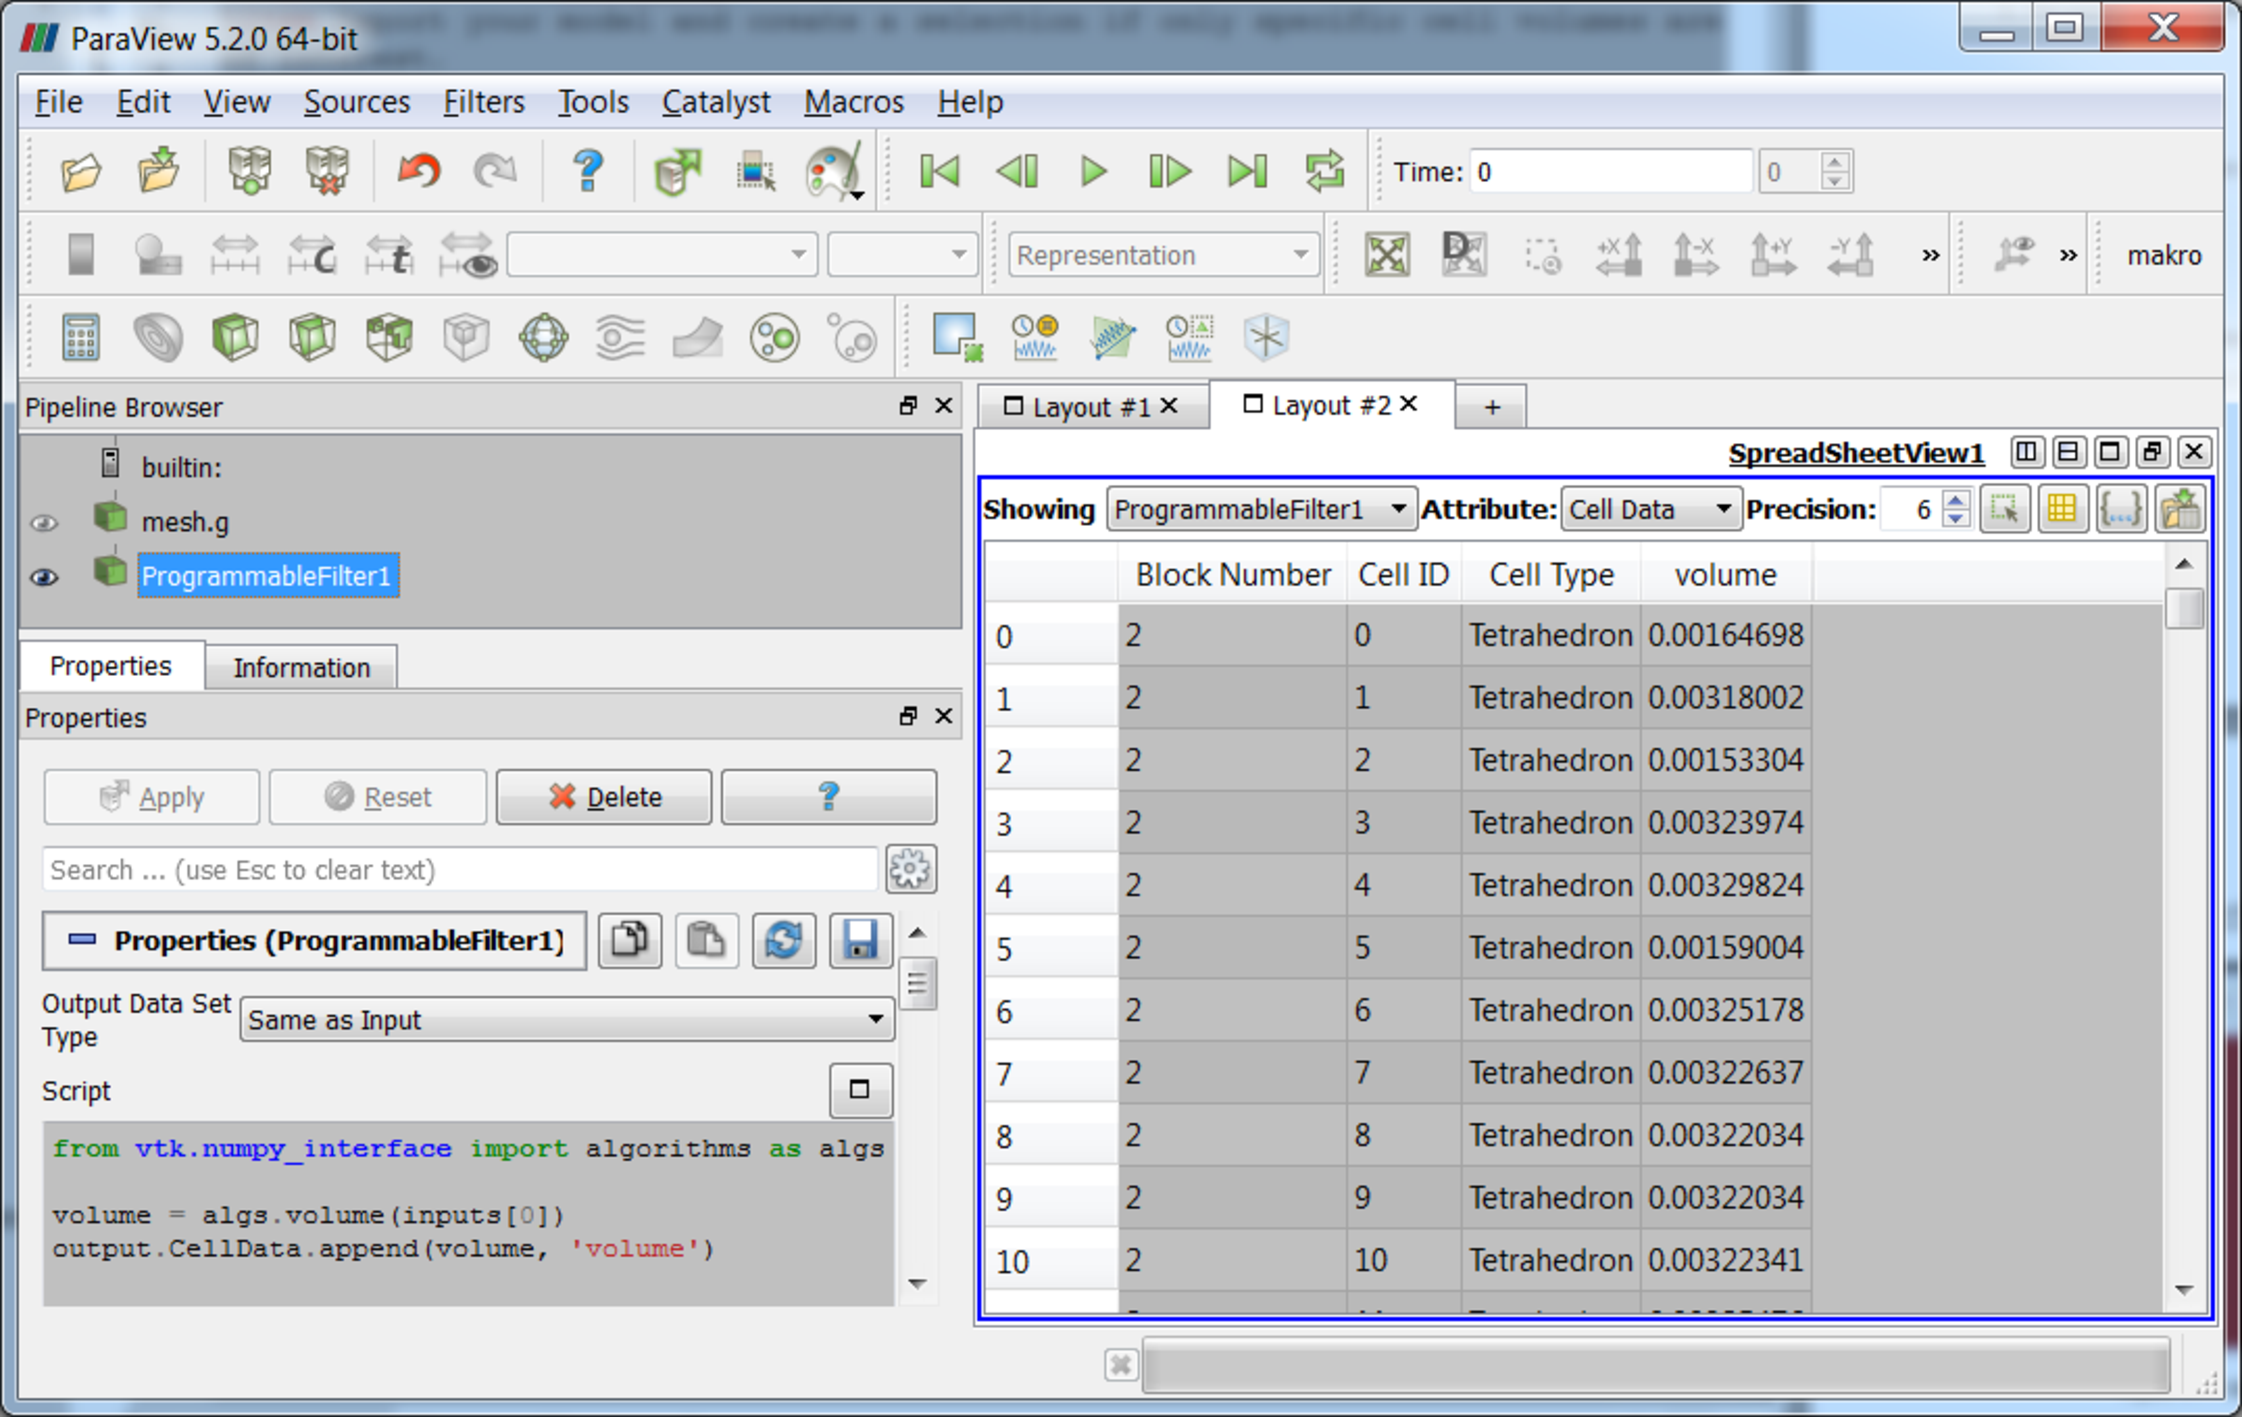
\includegraphics[width=\paraviewscreenshotwidthfac\linewidth]{Figures/Screenshots/ParaView_Calculate_Cell_Volume}
\caption{Display of cell volume calculation}
\label{fig:ParaView:Calculate:Cell:Volume}
\end{figure}